\documentclass[a4paper,french]{paper}
\usepackage{../../../../../_assets/latex/5N_OPTO_ELEC}

%Informations about this document 
%------------------------------------------
\def\module{Opto-Electronique - S5}
\def\moduleAbrege{5N-027-SCI / OptoElec}
\def\annee{2024-2025}

\def\titre{Séance 4 / Diodes}
\author{Julien VILLEMEJANE}

\subtitle{Séance 4}
\institution{LEnsE / Institut d'Optique Graduate School}

\title{\titre}
\begin{document} 
%Beginning First Page. 
%------------------------------------------
\enteteThematiqueObligatoire{}

\textit{Pour ce TD, on pourra s'appuyer sur la fiche résumée} : \href{https://lense.institutoptique.fr/ressources/Annee1/Electronique/fiches/2020_FR_Diodes_LED.pdf}{Diodes / LED / Photodiodes}

%Beginning Content. 

%%%%%%%%%%%%%%%%%%%
%%%%%%%%%%%%%%%%%%%
\encadreTDExo{4.1 - Limiter une tension}{
Rappeler le fonctionnement d'une diode.

Décrire le fonctionnement du montage suivant :

\begin{center}
\begin{circuitikz}
	\draw (0,0) to[battery2, invert] (0,5) to[short, -] (6,5)
		to[full diode=$D_1$, invert, i<_=$i_1$	] (6,2.5) to[full diode=$D_2$, invert, i<_=$i_2$, *-] (6,0)
		to[short, -*] (3,0) node[ground](GND){} to[short, -] (0,0);
	\draw (3,0) to[sV] (3,2.5) to[R=$R_p$, i=$i_R$] (6,2.5);
	\draw (6,2.5) to[short, -o] (8,2.5);
	\draw (8, 0) to[short, -o] ++(0,0) node[ground](GND){};
	\draw (8,0.3) edge[->,color={red}] (8, 2.2);
	\node[text={red}] (Vs) at (8.5,1.3){$V_S$}; 
	\draw (7,0.3) edge[<-,color={blue}] (7, 2.2);
	\node[text={blue}] (Vd2) at (7.5,1.3){$V_{D2}$}; 
	\draw (7,4.7) edge[->,color={blue}] (7, 2.8);
	\node[text={blue}] (Vd1) at (7.5,3.7){$V_{D1}$}; 
	\draw (2.5,0.3) edge[->,color={green!40!black}] (2.5, 2.2);
	\node[text={green!40!black}] (Ve) at (2,1.3){$V_e$}; 
	\draw (0.7,0.3) edge[->,color={black}] (0.7, 4.7);
	\node[text={black}] (Vcc) at (1.3, 2.5){$V_{CC}$}; 
\end{circuitikz}
\end{center}

}

%%%%%%%%%%%%%%%%%%%

Loi des mailles du circuit :

\begin{enumerate}
	\item $V_{CC} + V_{D1} + R_p \cdot i_R - V_E = 0$
	\item $-V_{D2} + R_p \cdot i_R - V_e = 0$
	\item $V_{D2} = -V_S$
\end{enumerate}

Les éléments $D_1$ et $D_2$ ont des caractéristiques tension-courant non linéaires.

\begin{center}
\begin{circuitikz}
	\draw (0,0) to[empty diode=$D$, i=$i_d$] (3,0);
	\draw (0,-1) edge[<-,color={blue}] (3, -1);
	\node[text={blue}] (Vd) at (1.5,-1.5){$u_d$}; 
\end{circuitikz}
\end{center}


On peut modéliser les diodes de la manière suivante :
\begin{itemize}
	\item si $u_D > V_F$, $i_d > 0$ et $u_d = V_F$
	\item sinon $i_d = 0$
\end{itemize}

$V_F$ est la tension directe (\textit{forward}) qui est un seuil de conduction dépendant du matériau utilisé. Cette valeur est fournie par le constructeur.

\bigskip

\textbf{Montage}

Comme il y a 2 éléments non linéaires dans le montage à étudier (et comme il y a peu de chance que les deux éléments conduisent ou soient bloquées en même temps), il y a 4 cas à traiter.

Nous allons partir d'une hypothèse sur la conduction des deux éléments et déterminer par la suite dans quelles conditions il est possible d'atteindre cet état.

\bigskip

\textbf{\textit{CAS 1}} $D_1$ et $D_2$ bloquées.

On a $i_1 = i_2 = 0$. Par la loi des noeuds entre les diodes on peut aussi en déduire que $i_r = i_1 + i_2 = 0$.

Ainsi, les lois des mailles 2 et 3 donnent : $V_S = V_E$.

\medskip

Pour être dans ce cas, il est impératif de vérifier les conditions suivantes : $V_{D1} < V_F$ (a) et $V_{D2} < V_F$ (b) (où $V_F$ est la tension seuil de conduction des diodes).

\medskip

\textit{Cas (a)}

$V_{D1} = V_E - V_{CC} - R_p \cdot i_R$ d'après 1

Ainsi $V_{D1} < V_F$ entraîne $V_E - V_{CC} < V_F$ et donc $$\boxed{V_E < V_{CC} + V_F}$$.

\medskip

\textit{Cas (b)}

$V_{D2} = - V_E + R_p \cdot i_R$ d'après 2

Ainsi $V_{D2} < V_F$ entraîne $- V_E < V_F$ et donc $$\boxed{V_E > - V_F}$$.

\medskip

Pour résumé, lorsque $ - V_F < V_e < V_{CC} + V_F $, les deux diodes sont bloquées et $V_S = V_E$.

\bigskip

\textbf{\textit{CAS 2}} $D_1$ bloquée et $D_2$ passante

On a $i_1 = 0$ mais $i_2 \neq 0$. Par la loi des noeuds entre les diodes on peut aussi en déduire que $i_r = -i_2$.

De plus, $V_{D2} = V_F$. D'après 3, on a alors $$\boxed{V_S = -V_F}$$

Cette condition est réalisée lorsque $V_{D2} > V_F$, ce qui entraîne $- V_E > V_F$ et donc $$\boxed{V_E < - V_F}$$.

On peut vérifier que dans cette condition, $D_1$ est bien bloquée.

\bigskip

\textbf{\textit{CAS 3}} $D_1$ passante et $D_2$ bloquée

On a $i_1 \neq 0$ mais $i_2 = 0$. Par la loi des noeuds entre les diodes on peut aussi en déduire que $i_r = i_1$.

De plus, $V_{D1} = V_F$. D'après 1, on a alors $$\boxed{V_S = V_{CC} + V_F}$$

Cette condition est réalisée lorsque $V_{D1} > V_F$, ce qui entraîne $V_E - V_{CC} > V_F$ et donc $$\boxed{V_E > V_{CC} + V_F}$$.

On peut également vérifier que dans cette condition, $D_2$ est bien bloquée.

\bigskip

\textbf{\textit{CAS 4}} $D_1$ et $D_2$ passantes

Ce cas est impossible, d'après les conditions calculées dans le cas 1 (si $V_{CC}$ est strictement positif).



%%%%%%%%%%%%%%%%%%%
%%%%%%%%%%%%%%%%%%%
\encadreTDExo{4.2 - Réguler une tension}{
Soit le montage suivant : 
 
 
\begin{center}
\begin{circuitikz}
	\draw (0,0) node[ground]{} 
		to[empty Zener diode=$D_Z$, i=$i_d$, -*] (0,2.5)
		to[R=$R_0$, i<_=$i_0$] (0,5)
		to[short, -] (-2,5)
		to[battery2] (-2,0)
		to[short,-*] (0,0);
	\draw[dashed] (0,2.5) to[short, -o, i=$i_s$] (2,2.5);
	\draw[dashed] (0,0) to[short, -o] (2,0);
	\draw (2,0.3) edge[<-,color={blue}] (2, 2.2);
	\node[text={blue}] (Vd) at (2.5,1.2){$u_d$};
	\draw (3,0.3) edge[->,color={red}] (3, 2.2);
	\node[text={red}] (Vs) at (3.5,1.2){$V_S$};
	\draw (-1.5,0.3) edge[->,color={black}] (-1.5, 4.7);
	\node[text={black}] (Vcc) at (-1,2.5){$V_{CC}$};
\end{circuitikz}
\end{center}

On donne une partie de la documentation d'une diode Zener de type 1N47xxA.

Expliquez le rôle de ce montage.

}


%%%%%%%%%%%%%%%%%%%
\textbf{Diode Zener}

Une diode Zener est un composant non linéaire, qui possède deux zones "passantes", contrairement à des diodes de signal plus classiques qui ne possède qu'une zone "passante" pour des tensions positives (voir caractéristique ci-dessous).

\begin{center}
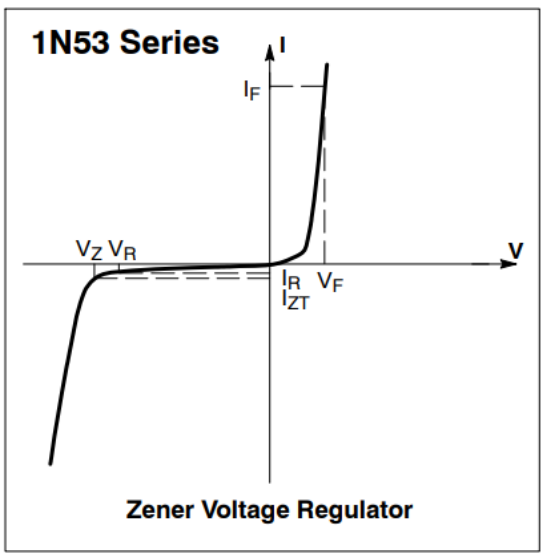
\includegraphics[width=6cm]{images/zener_carac.png}
\end{center}

\begin{center}
\begin{circuitikz}
	\draw (0,0) to[empty Zener diode=$D_Z$, i=$i_d$] (3,0);
	\draw (0,-1) edge[<-,color={blue}] (3, -1);
	\node[text={blue}] (Vd) at (1.5,-1.5){$u_d$}; 
\end{circuitikz}
\end{center}

Il existe alors deux limites de conduction :
\begin{itemize}
	\item si $u_d > V_F$, alors $i_d > 0$ (sens direct)
	\item si $u_d < - V_Z$, alors $i_d < 0$ (sens Zener)
	\item sinon $i_d = 0$
\end{itemize}

\textbf{Montage Zener}

\begin{center}
\begin{circuitikz}
	\draw (0,0) node[ground]{} 
		to[empty Zener diode=$D_Z$, i=$i_d$, -*] (0,2.5)
		to[R=$R_0$, i<_=$i_0$] (0,5)
		to[short, -] (-2,5)
		to[battery2] (-2,0)
		to[short,-*] (0,0);
	\draw[dashed] (0,2.5) to[short, -o, i=$i_s$] (2,2.5);
	\draw[dashed] (0,0) to[short, -o] (2,0);
	\draw (2,0.3) edge[<-,color={blue}] (2, 2.2);
	\node[text={blue}] (Vd) at (2.5,1.2){$u_d$};
	\draw (3,0.3) edge[->,color={red}] (3, 2.2);
	\node[text={red}] (Vs) at (3.5,1.2){$V_S$};
	\draw (-1.5,0.3) edge[->,color={black}] (-1.5, 4.7);
	\node[text={black}] (Vcc) at (-1,2.5){$V_{CC}$};
\end{circuitikz}
\end{center}

Loi des mailles : $V_{CC} - R_0 \cdot i_0 + u_d = 0$

Ainsi : $u_d = R_0 \cdot i_0 - V_{CC}$

\textbf{\textit{Cas 1 (sens direct)}}

Pour que la diode soit passante dans le sens direct, il faut que $u_d > V_F$, c'est à dire que $R_0 \cdot i_0 - V_{CC} > V_F$.

On obtient alors, à la limite de conduction (lorsque $i_0 = 0^+$), la condition que $V_{CC} < -V_F$.

Par principe $V_{CC}$ sera positif. Ce cas est donc impossible.


\textbf{\textit{Cas 2 (sens Zener)}}

Pour que la diode soit passante dans le sens Zener, il faut que $u_d < -V_Z$, c'est à dire que $R_0 \cdot i_0 - V_{CC} < -V_Z$.

On obtient alors, à la limite de conduction (lorsque $i_0 = 0^+$), la condition que $V_{CC} > V_Z$. Dans cette condition, $u_d = -V_Z$ et donc $V_S = -u_d = V_Z$ !

Dans cette condition, la tension $V_S$ de ce montage est (quasi)constante et égale à la tension Zener.

On obtient un \textbf{régulateur de tension}.


%%%%%%%%%%%%%%%%%%%
%%%%%%%%%%%%%%%%%%%
\encadreTDExo{4.3 - Redresser une tension}{

Soient les circuits suivants :

\begin{center}
	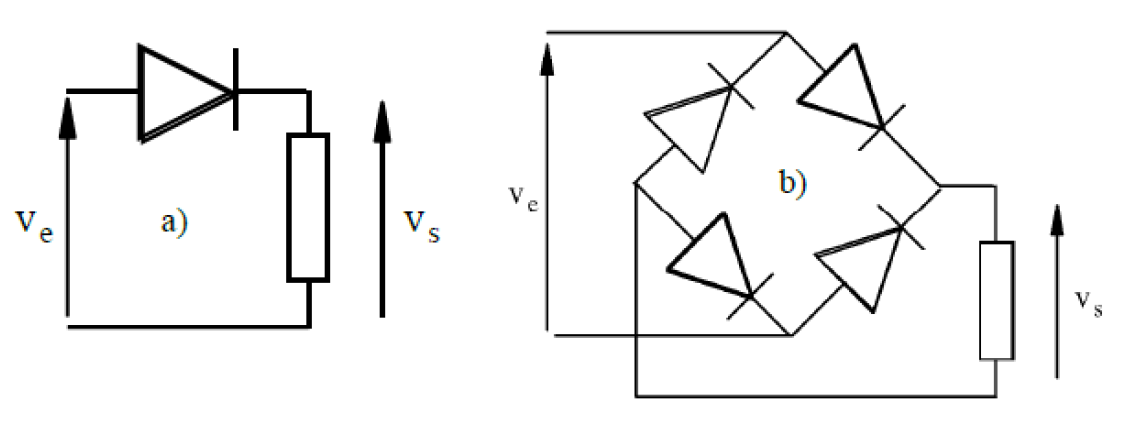
\includegraphics[width=8cm]{images/redresseur_001_a.png}
\end{center}

Donnez l'allure du signal de sortie $V_S(t)$ des circuits a et b suivants pour un signal d'entrée de forme sinusoïdale telle que $V_e(t) = A \cdot sin(\omega{}t)$ dans le cas d'une diode idéale. Puis dans le cas d'une diode avec une tension de seuil $V_d$. On supposera que $A > V_d$.

}

%%%%%%%%%%%%%%%%%%%

\begin{center}
	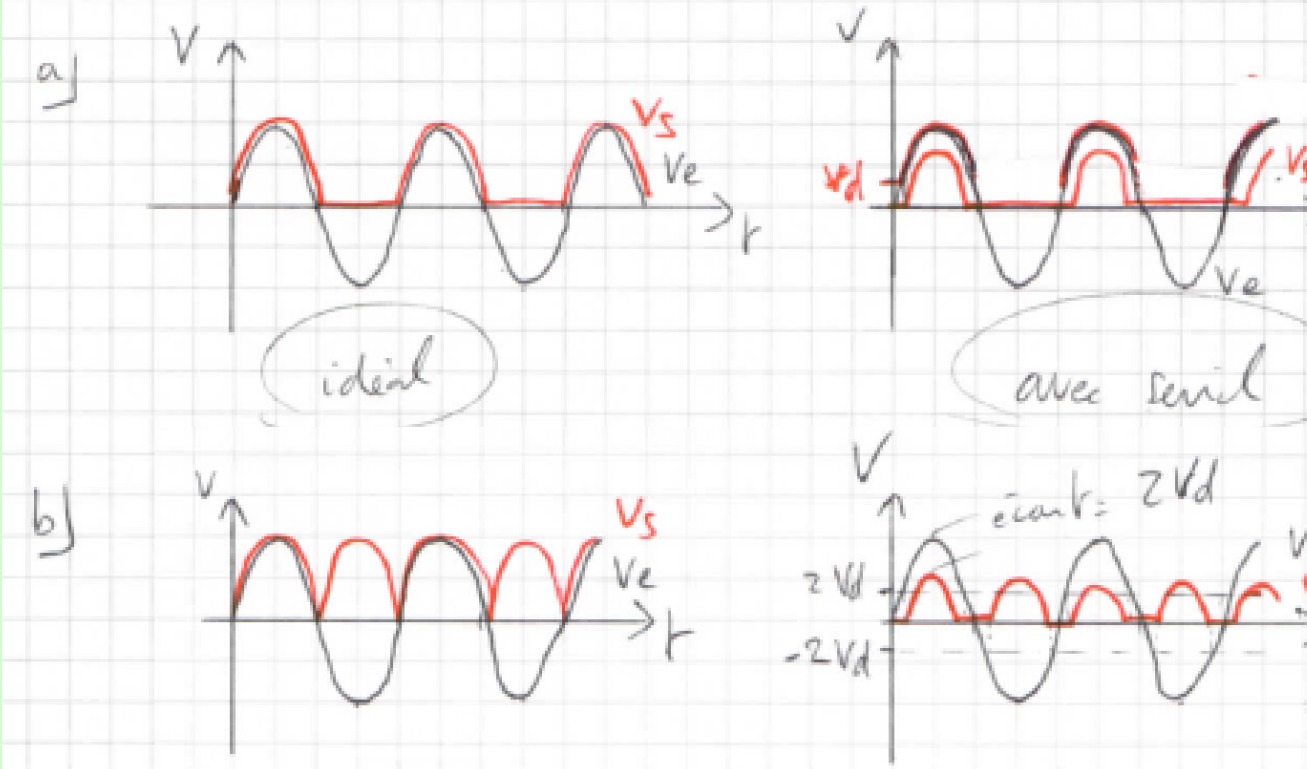
\includegraphics[width=8cm]{images/redresseur_001_a_cor.png}
\end{center}
	
On peut également simuler ce montage (à l'aide du logiciel LTSpice par exemple). On obtient alors, dans le cas d'une diode "classique", la figure suivante - cas (a) à gauche et cas (b) à droite ($A = 10\operatorname{V}$ et $f = 10\operatorname{Hz}$ - en haut les tensions $V_E(t)$ et $V_S(t)$ et en bas le courant dans la diode pour le cas (a) et dans la résistance R pour le cas (b)) :

\begin{center}
	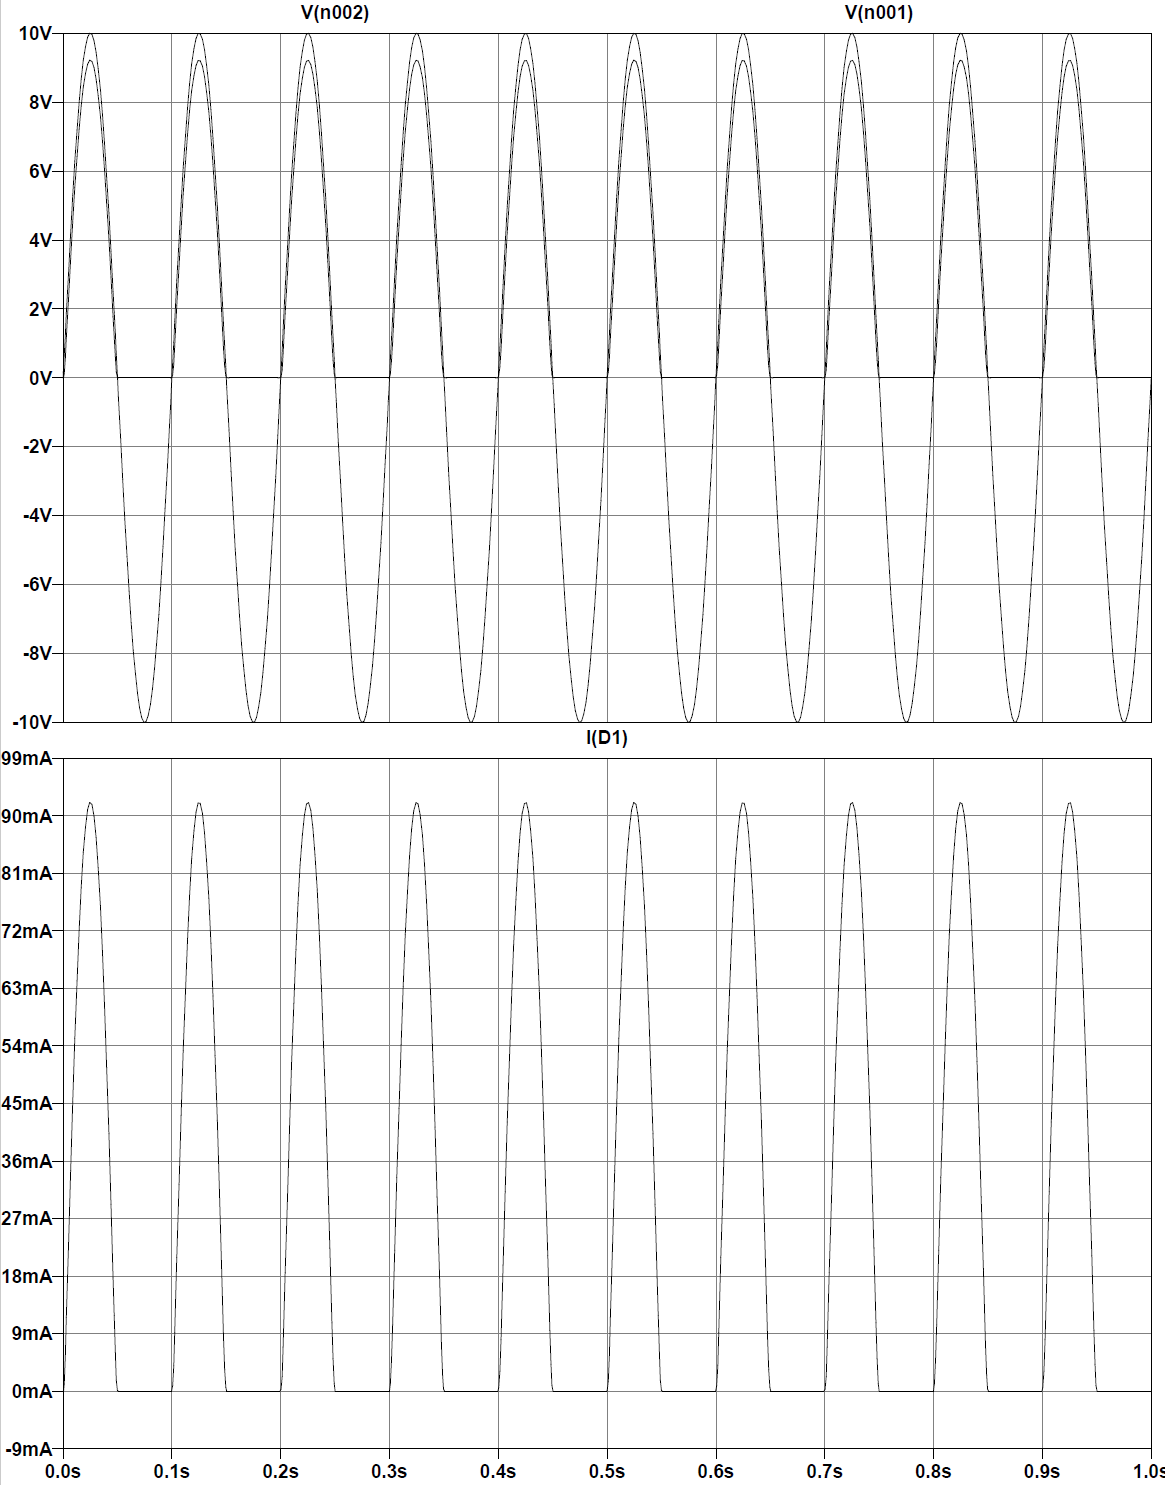
\includegraphics[width=6cm]{images/redresseur_001_b_cor.png}\hfill
	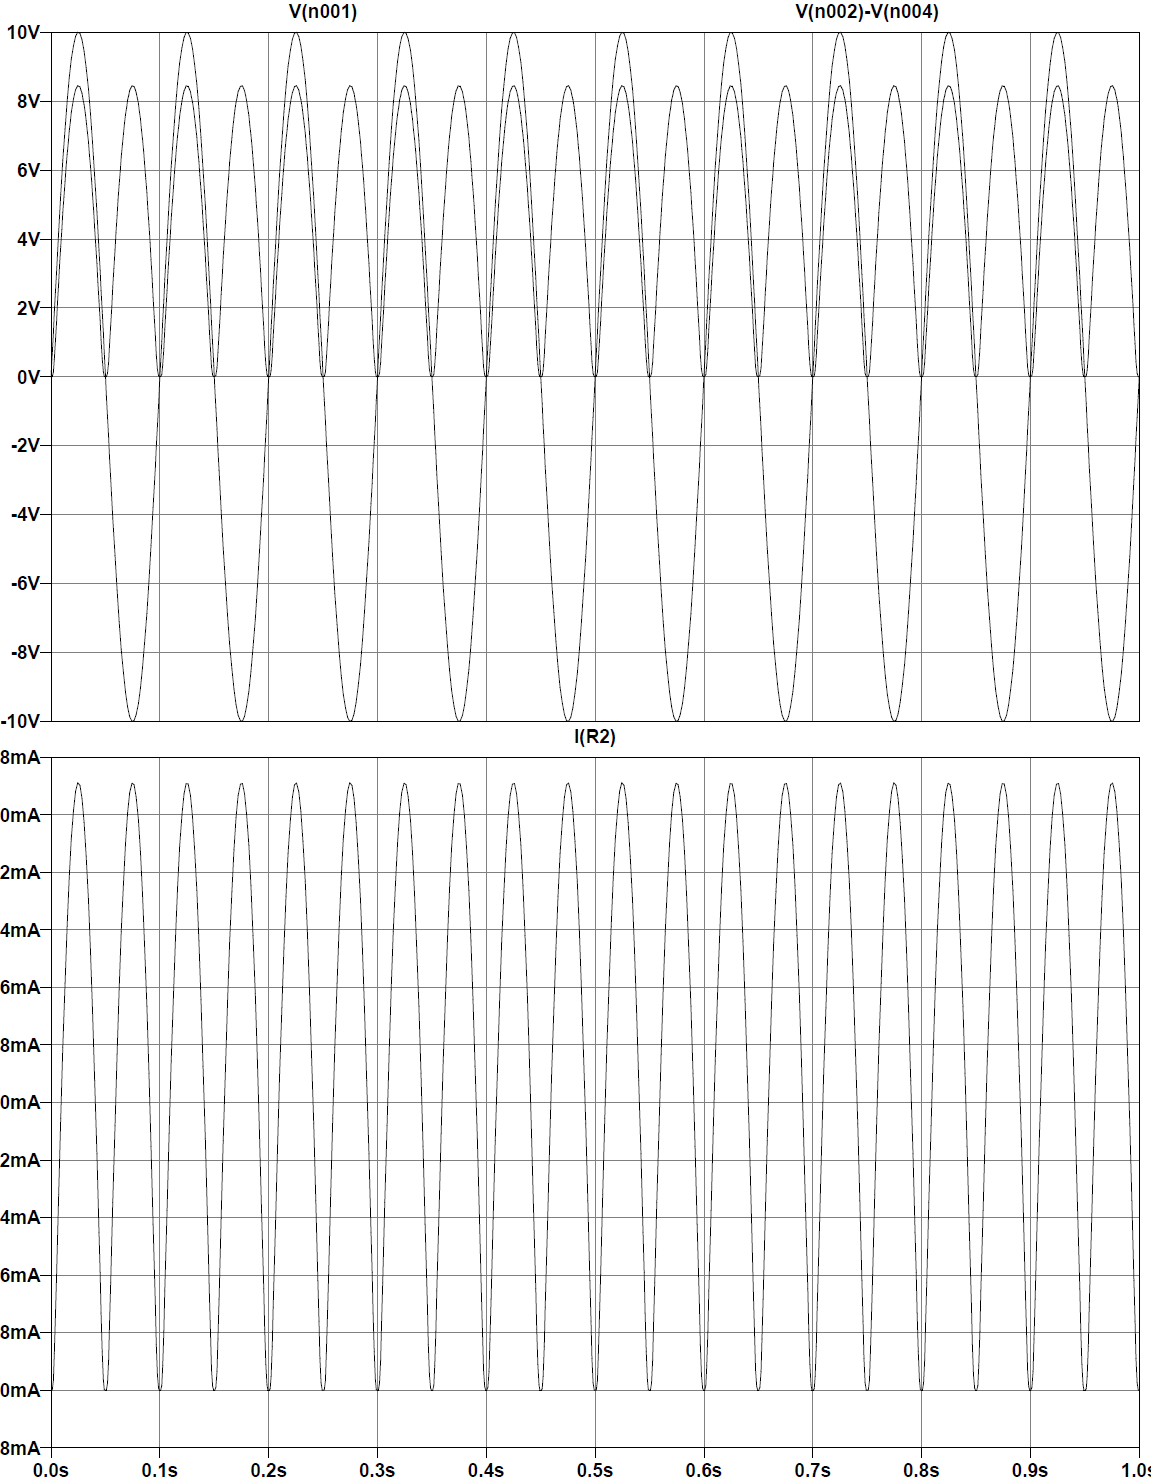
\includegraphics[width=6cm]{images/redresseur_001_c_cor.png}
\end{center}	
	
	
%%%%%%%%%%%%%%%%%%%
%%%%%%%%%%%%%%%%%%%
\encadreTDExo{4.4 - Modifier la forme d'une tension}{

On considère les deux montages suivants :

\begin{center}
	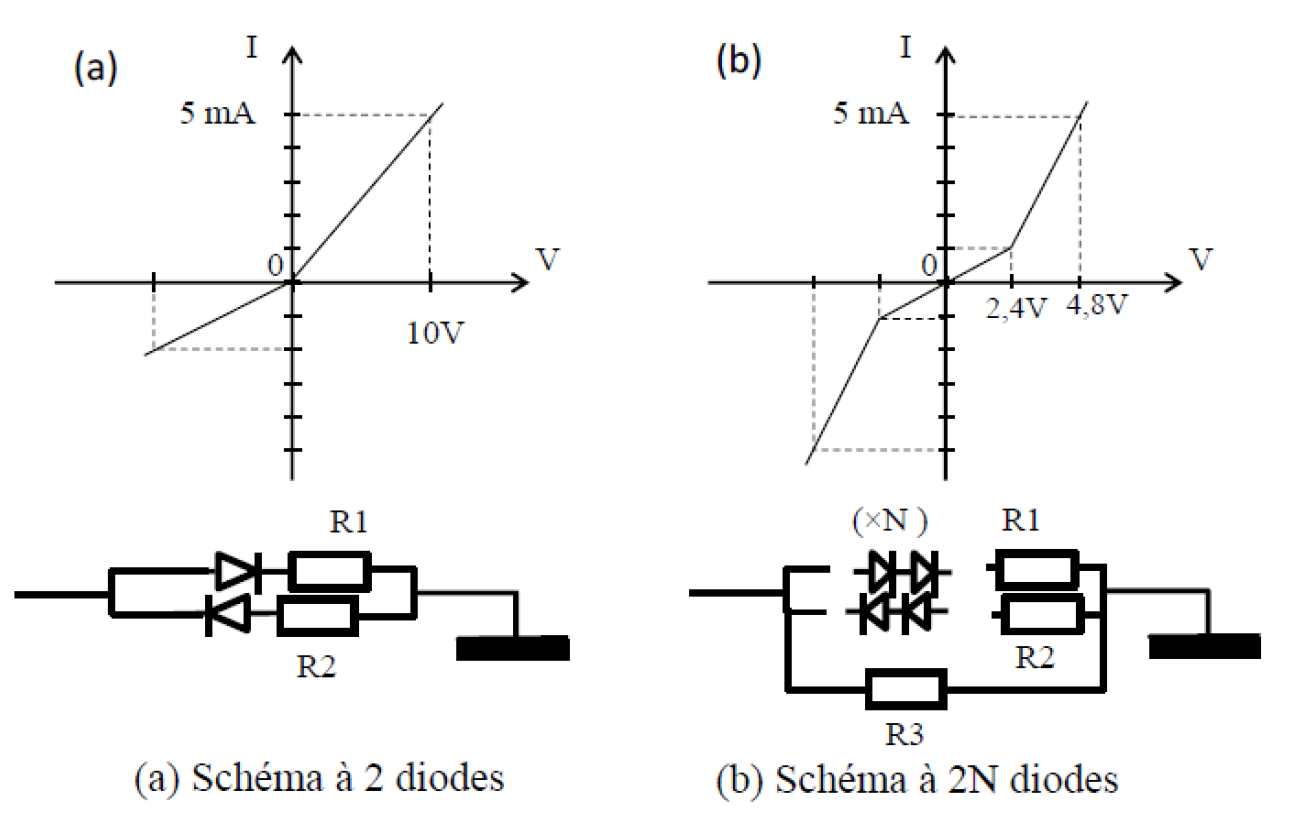
\includegraphics[width=12cm]{images/diodes_002_a.png}
\end{center}

\begin{enumerate}
	\item Dans le cas du montage de la figure (a) et d'utilisation de diodes parfaites et idéales, que doivent valoir $R_1$ et $R_2$ pour obtenir la caractéristique tracée dans le graphe $I(V)$ ?
	\item Dans le cas du montage de la figure (b), les diodes ont pour seuil $0,6\operatorname{V}$. Que doivent valoir $R_1$, $R_2$ et $R_3$ et le nombre de diodes $N$ ($N = 2$ a été dessiné arbitrairement) pour obtenir la caractéristique tracée dans le graphe $I(V)$ ?
\end{enumerate}
}

\textbf{Question 1 / Montage a}
	
$R_1$ donne la pente lorsque $V < 0$, on a alors : $R_1 = \Delta{}V=\Delta{}I = 10/5 \cdot 10^{-3} = 2\operatorname{k\Omega}$

De même, $R_2$ donne la pente lorsque $V > 0$, on a alors : $R_2 = \Delta{}V=\Delta{}I = 10/2 \cdot 10^{-3} = 5\operatorname{k\Omega}$

\textbf{Question 1 / Montage b}
	
Entre $-2.4\operatorname{V}$ et $+2.4\operatorname{V}$, seule la résistance $R_3$ intervient, les diodes des autres branches sont bloquées. On a alors : $R3 = \Delta{}V=\Delta{}I = 2.4 / 10^{-3} = 2.4\operatorname{k\Omega}$

\medskip

Pour un changement de comportement à $+2.4\operatorname{V}$, il faut au total $N = 4$ diodes en série ($4 \cdot 0.6\operatorname{V} = 2.4\operatorname{V}$).

\medskip

Les pentes avant $-2.4\operatorname{V}$ et après $2.4\operatorname{V}$ étant les mêmes, $R_1 = R_2$

De plus, dans cette zone-là, $R_1 // R_3 = R_1 \cdot R_3 / (R_1 + R_3) = \Delta{}V=\Delta{}I = 2.4 / 4 \cdot 10^{-3} = 600\operatorname{\Omega}$

Ainsi, $R_1 = 800\operatorname{\Omega}$.



%%%%%%%%%%%%%%%%%%%
%%%%%%%%%%%%%%%%%%%
\encadreTDExo{4.B1 - Emettre des photons à partir d'une LED}{

On souhaite réaliser un montage émetteur à l'aide d'une \textbf{diode rouge} de type KingBright L-53HD. On propose d'étudier le montage suivant :

\begin{center}
	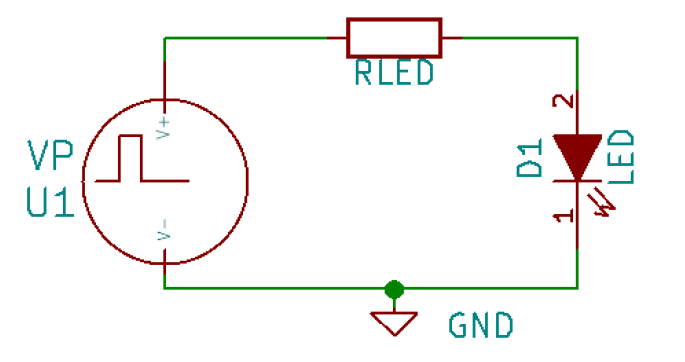
\includegraphics[width=8cm]{images/emetteur_003_a.png}
\end{center}

On donne une partie de la documentation : 

\begin{center}
	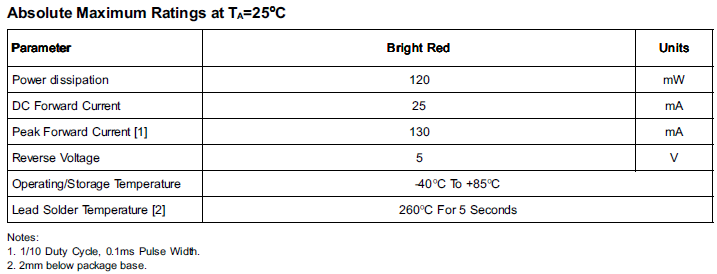
\includegraphics[width=14cm]{images/doc_led_rouge.png}
\end{center}

\begin{enumerate}
	\item Cas 1 : La source de tension $V_P$ est une \textbf{source continue}. Elle délivre une différence de potentiel de $5\operatorname{V}$.
	\begin{enumerate}
		\item Quelle est la valeur maximale du courant que la diode peut supporter dans ces conditions ?
		\item Quelle est la valeur minimale que doit avoir $R_{LED}$ pour respecter cette condition ?
		\item Quel sera alors le courant moyen qui traversera la LED ?
	\end{enumerate}
	
	\item Cas 2 : La source de tension $V_P$ est une \textbf{source impulsionnelle}. Elle délivre des impulsions de $5\operatorname{V}$ de durée $0.1\operatorname{ms}$ avec une fréquence de répétition de $1\operatorname{kHz}$.
	\begin{enumerate}
		\item Quelle est la valeur maximale du courant que la diode peut supporter dans ces conditions ?
		\item Quelle est la valeur minimale que doit avoir $R_{LED}$ pour respecter cette condition ?
		\item Quel sera alors le courant moyen qui traversera la LED ?
	\end{enumerate}
\end{enumerate}
}


%%%%%%%%%%%%%%%%%%%
\centerline {\rule{.5\linewidth}{.25pt}} % Horizontal line
\textbf{\large Cas 1}

\textbf{Question 1.a}

Une tension continu (et donc un courant continu) sera appliqué sur la LED dans les conditions décrites. Ainsi, la donnée qui nous intéresse est le courant direct maximal (ou \textit{DC Forward Current}). $I_{FMAXDC} = 25\operatorname{mA}$.



\textbf{Question 1.b}
	
Lorsque la diode est passante, elle est soumise à une différence de potentiel nommée tension directe ou $V_F$ (\textit{Forward Voltage}). Cette différence de potentiel est donnée pour un courant continu de 20~mA. $V_F = 2.5\operatorname{V}$.

La loi des mailles donne ensuite : $V_P = R_{LED} \cdot I_F + V_F$. On a alors le courant $I_F$ qui vaut : $I_F = \frac{V_P - V_F}{R_{LED}}$.

Or on souhaite que $I_F < I_{FMAXDC}$. On obtient alors que $$R_{LED} > \frac{V_P - V_F}{I_{FMAXDC}} = 100\operatorname{\Omega}$$.


\textbf{Question 1.c}

$<I_F> = I_{FMAXDC}$

%%%%%%%%%%%%%%%%%%%
\centerline {\rule{.5\linewidth}{.25pt}} % Horizontal line
\textbf{\large Cas 2}

\textbf{Question 2.a}
	
La durée de l'impulsion délivrée est $t_{on} = 0.1\operatorname{ms}$. La période du signal est $T = 1/f = 1\operatorname{ms}$. Le rapport cyclique vaut alors $D = \frac{t_{on}}{T} = 0.1$.

D'après la documentation technique, dans ces conditions d'utilisation, il est possible d'utiliser un courant plus important, la LED ayant le temps entre deux impulsions de "refroidir". Ainsi, le courant $I_{FMAX} = 130\operatorname{mA}$.


\textbf{Question 2.b}
	
De la même manière que précédemment, on a $R_{LED} > \frac{V_P - V_F}{I_{FMAX}} = 19\operatorname{\Omega}$

\textbf{Question 2.c}

$\displaystyle <I_F> = \int_{0}^{T} i(t) \, \mathrm{d}t = D \cdot I_{FMAX} = 13\operatorname{mA}$



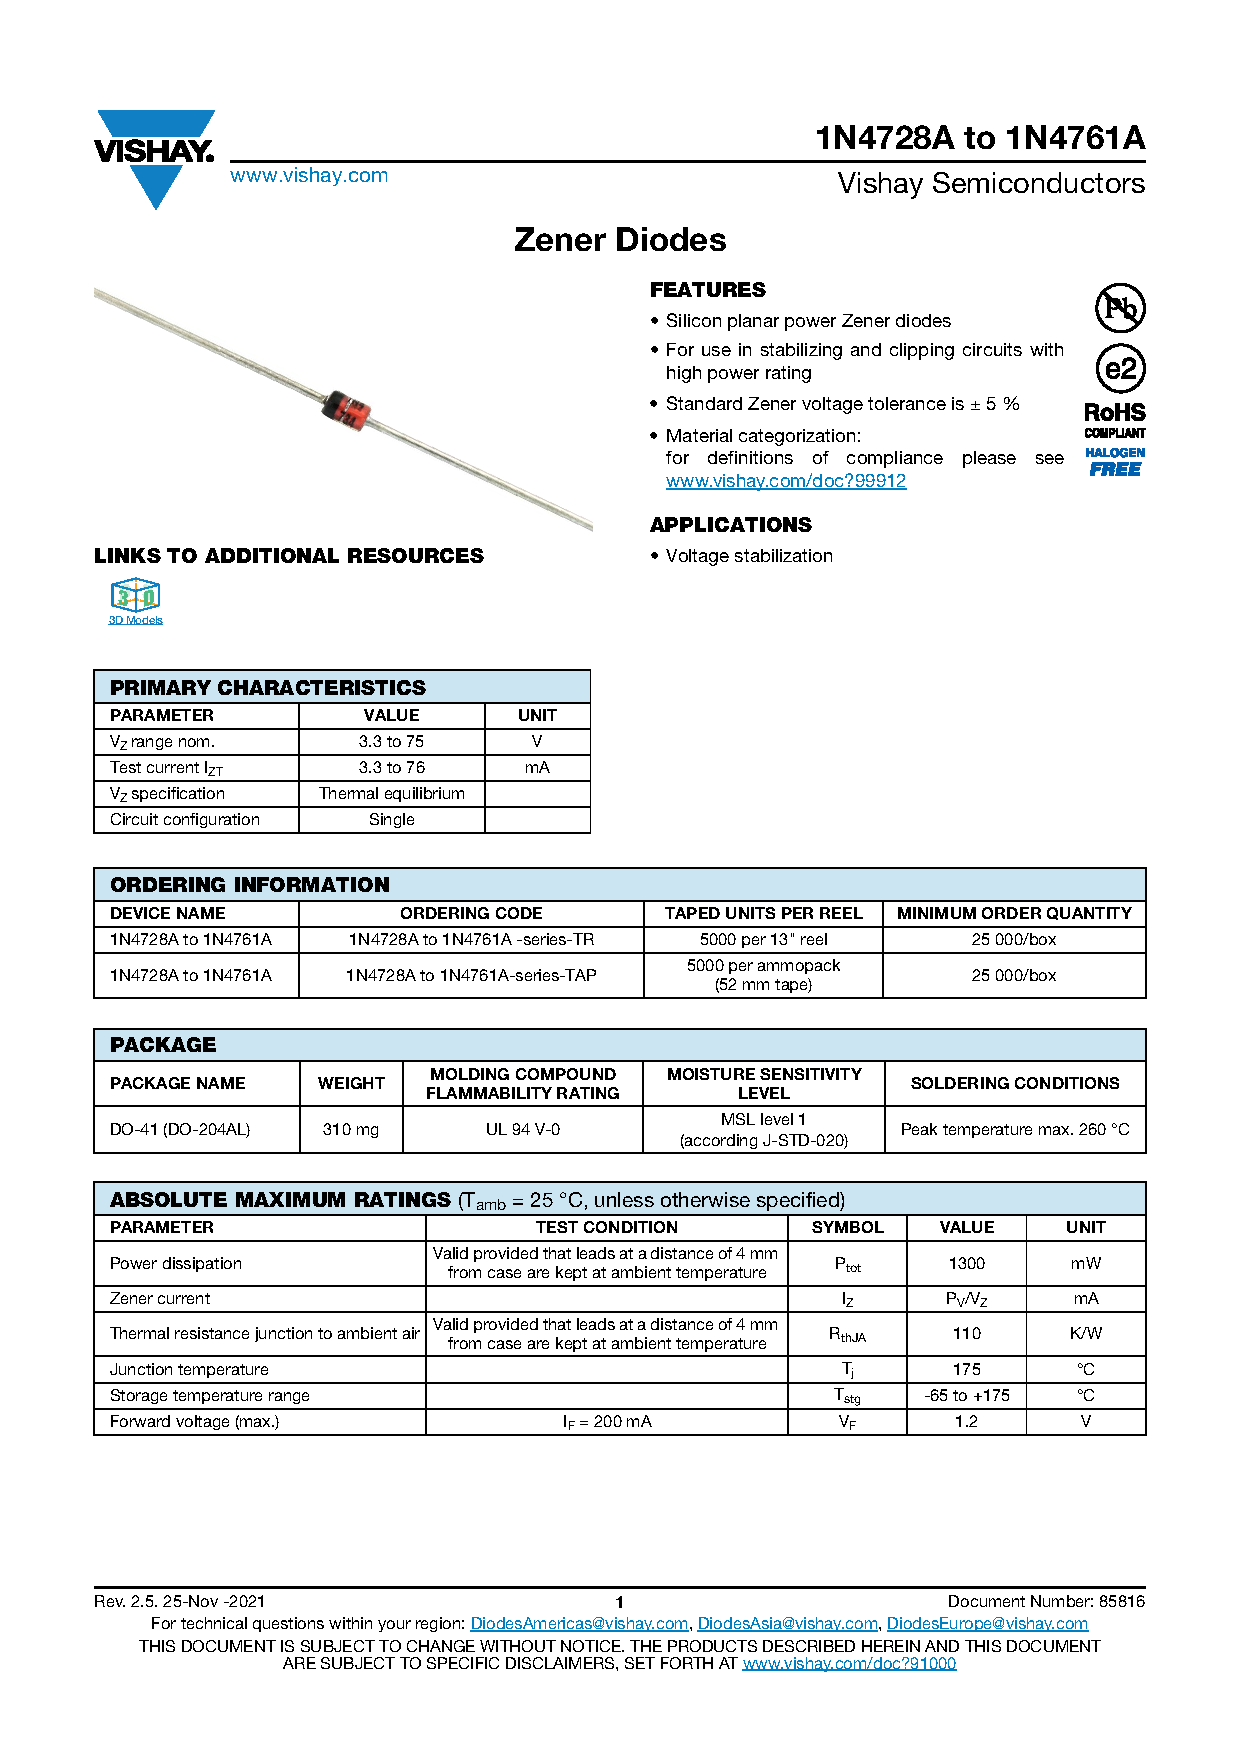
\includepdf[pages=1-2]{docs/1n4728a.pdf}

\end {document}